\documentclass[]{article}
\usepackage{graphicx}
\usepackage[space]{grffile}
\usepackage{subfig}
\graphicspath{ {./roc_curves/} }

%opening
\title{Transfer Learning Using Convolutional Neural Networks to Detect Spoofs in Fingerprints}
\author{Chris Denniston}

\begin{document}

\maketitle

\begin{abstract}
% This should be a snap-shot of the whole paper, in 200 words or less. Start with a couple of sentences summarizing S1 (please see below), a short but precise summery of data and the utilized computational methods (e.g. different auto-encoderand NN classifiers used), and then finish by the most representative results (include figures) and one sentence on your main conclusion.
\end{abstract}
\textit{This paper was written by the author in their own words and all external knowledge and literature has been referenced properly in it's respective text.}
\section{Introduction}
%S1-Introduction (What and Why)
%A short description of the dataset, followed by a couple of paragraphs about importance of deep learning and its applications.
%1-What (precise problem statement)
%2-Why (importance of the subject matter, AND importance of your approach: is it new? more accurate? more efficient?)
Detection of impostor fingerprints are an important part of a fingerprint based biometric system. These impostor and fake fingerprints are commonly called "spoofs" It is not enough that the system can tell apart one person from another, but also must be able to tell apart fake fingerprints from real fingerprints to inspire real confidence in it's users. Spoof fingerprints can be made from common household materials and more and more material's are appearing which can be used to make these spoofs. Because of this it is also important that a spoof detection system also can detect spoofs when novel types of materials are used on it. 

A neural network may be used to solve this complex classification problem as it has the ability to learn from a large variety of samples and draw complex decision boundaries. \cite{book} (Citation?) Neural networks are expensive to train for complex problems involving large dimensional data, such as images. It is possible to take a pre-trained general image classification neural network and reapply it to this classification task. This enables a much quicker training time and more accurate results than could be achieved by a small team. 

Convolutional Neural Networks provide a framework 
\section{Methods}
%Precisely and concisely describe data preparation and classification methods you used. %Write at least one paragraph for each method, accompanied by corresponding
%reference. Put formulas in the appendix.
%3-How (your data and methods, described to the level that your experiment is reproducible by your audience)
\section{Results}
%This section presents the detailed results you have obtained. If the paper is theoretical, you will probably show curves obtained from your equations. If the paper is experimental, you will be presenting curves showing the measurement results. In order to choose the proper curves to present, you must first be clear what point you are trying to convey to the reader. The curves can then be chosen to illustrate this point. Whether your paper is theoretical or experimental, you must provide a careful interpretation of what your results mean and why they behave as they do.
%This is the main part of your paper and should constitute about 40%-50% of its length.
%Cogently write down, discuss, and justify the results of your experiments and
%observations from all the cases you tried for your project: what types and ranges of
%classification parameters did you try in each case, and why? What trends did you see?
%You need to justify and explain everything referring to the basic concepts and theory
%taught in class, citing relevant references from your textbook or earlier mentioned
%references (use page numbers and section names in addition to the standard
%reference). Elucidate your point by referring to corresponding enumerated tables, figures, and formulas in the appendix.

\section{Conclusion}
%Section IV: Conclusion This section should summarize what has been accomplished in the paper. Many readers will read only the Introduction and Conclusion of your paper. The Conclusion should be written so they can be understood by someone who has not read the main work of the paper.
%Start by a complete summary of your work, and finish by your major conclusions andtake home messages (e.g. on the capabilities and limitations of the used methods givenyour project experience).

\section{Reference}
\bibliographystyle{ieeetr}
\bibliography{/home/octopuscabbage/code/NeuralAndAdaptiveSystemsFinal/report/bib.bib}
\section{Appendix}
\begin{figure}[!ht]
     \subfloat[Testing\label{subfig-1:dummy}]{%
       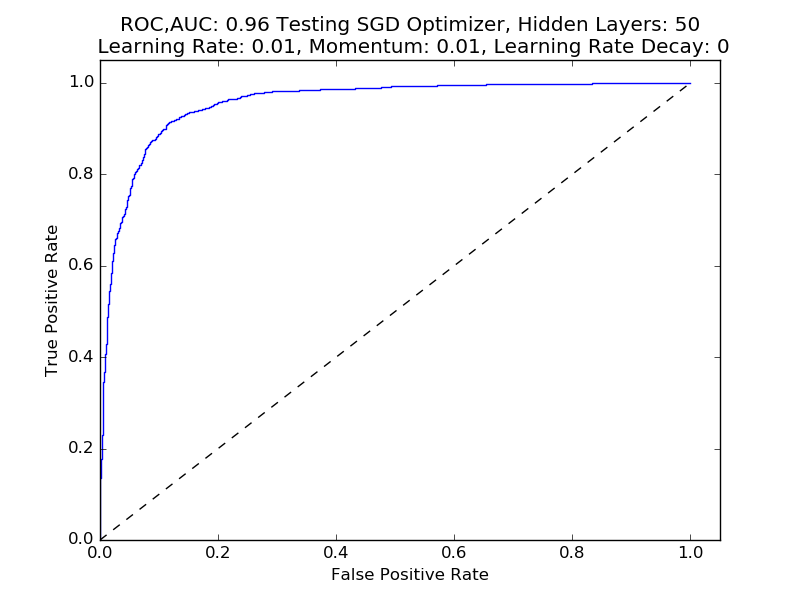
\includegraphics[width=0.5\textwidth]{/home/octopuscabbage/code/NeuralAndAdaptiveSystemsFinal/roc_curves/SGD Optimizer, Hidden Layers: 50 Learning Rate: 0.01, Momentum: 0.01, Learning Rate Decay: 0/ROC,AUC: 0.96 Testing SGD Optimizer, Hidden Layers: 50 Learning Rate: 0.01, Momentum: 0.01, Learning Rate Decay: 0}
     }
     \hfill
     \subfloat[Validation\label{subfig-2:dummy}]{%
       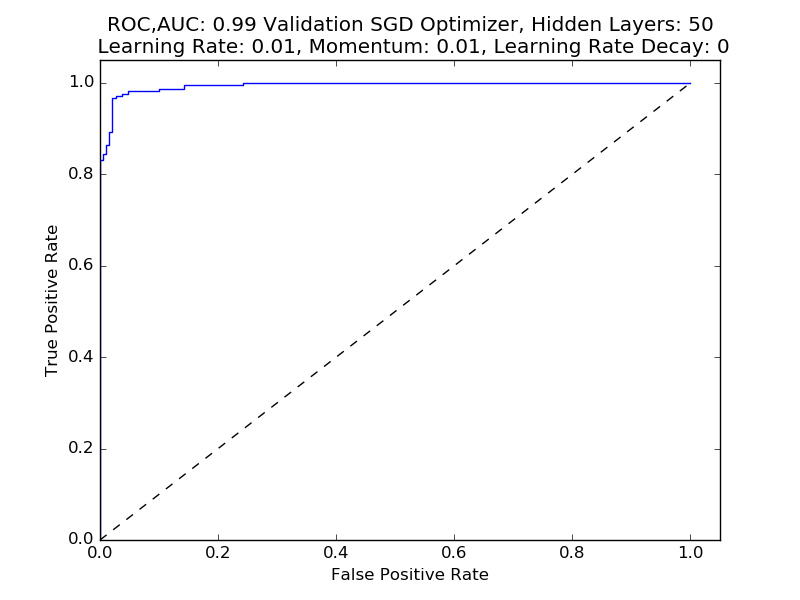
\includegraphics[width=0.5\textwidth]{/home/octopuscabbage/code/NeuralAndAdaptiveSystemsFinal/roc_curves/SGD Optimizer, Hidden Layers: 50 Learning Rate: 0.01, Momentum: 0.01, Learning Rate Decay: 0/ROC,AUC: 0.99 Validation SGD Optimizer, Hidden Layers: 50 Learning Rate: 0.01, Momentum: 0.01, Learning Rate Decay: 0}
     }
     \caption{ROC Curves For Training On All Samples}
     \label{fig:dummy}
   \end{figure}

\begin{figure}[!ht]
     \subfloat[Gelatine\label{subfig-3:dummy}]{%
       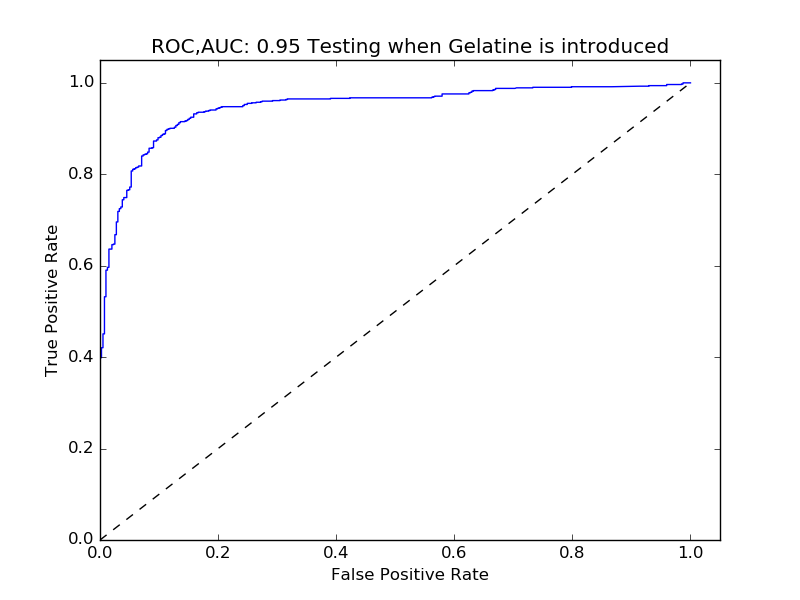
\includegraphics[width=0.5\textwidth]{/home/octopuscabbage/code/NeuralAndAdaptiveSystemsFinal/roc_curves/Gelatine/ROC,AUC: 0.95 Testing when Gelatine is introduced}
     }
     \hfill
     \subfloat[Latex\label{subfig-4:dummy}]{%
       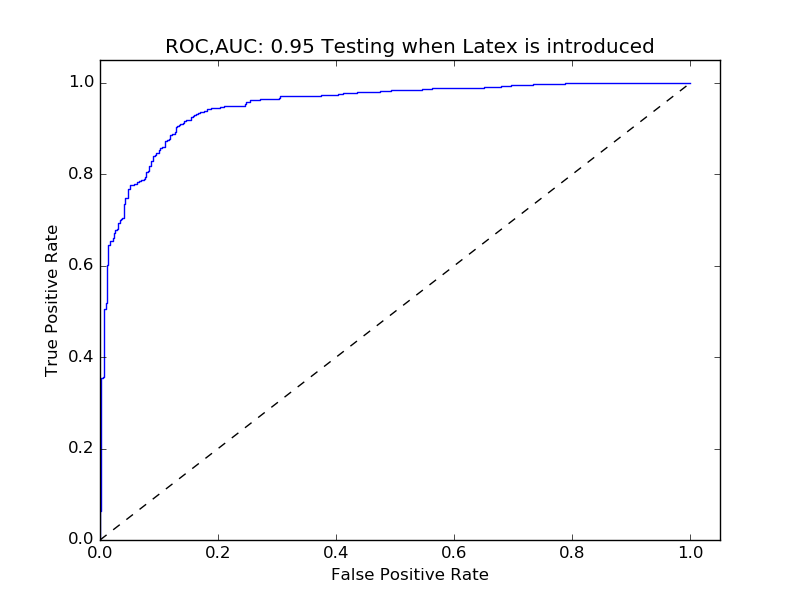
\includegraphics[width=0.5\textwidth]{/home/octopuscabbage/code/NeuralAndAdaptiveSystemsFinal/roc_curves/Latex/ROC,AUC: 0.95 Testing when Latex is introduced}
     }
     \hfill
     \subfloat[Playdoh\label{subfig-5:dummy}]{%
            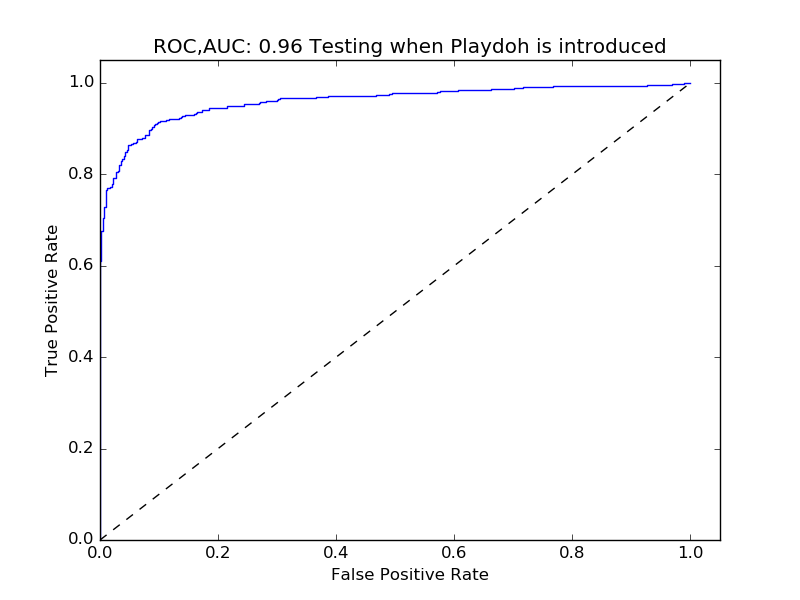
\includegraphics[width=0.5\textwidth]{/home/octopuscabbage/code/NeuralAndAdaptiveSystemsFinal/roc_curves/Playdoh/ROC,AUC: 0.96 Testing when Playdoh is introduced}
    }
    \hfill
    \subfloat[Silicone\label{subfig-6:dummy}]{%
    	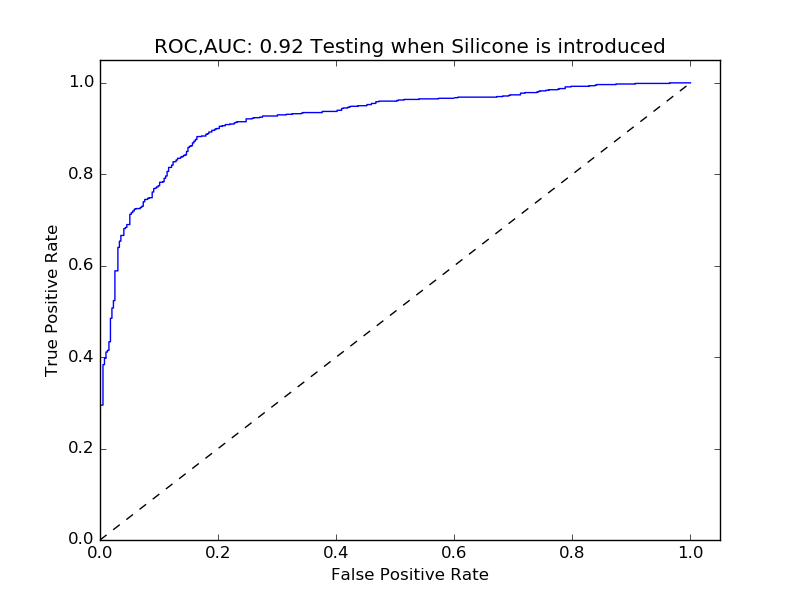
\includegraphics[width=0.5\textwidth]{/home/octopuscabbage/code/NeuralAndAdaptiveSystemsFinal/roc_curves/Silicone/ROC,AUC: 0.92 Testing when Silicone is introduced}
    }
    \subfloat[Wood Glue\label{subfig-7:dummy}]{%
         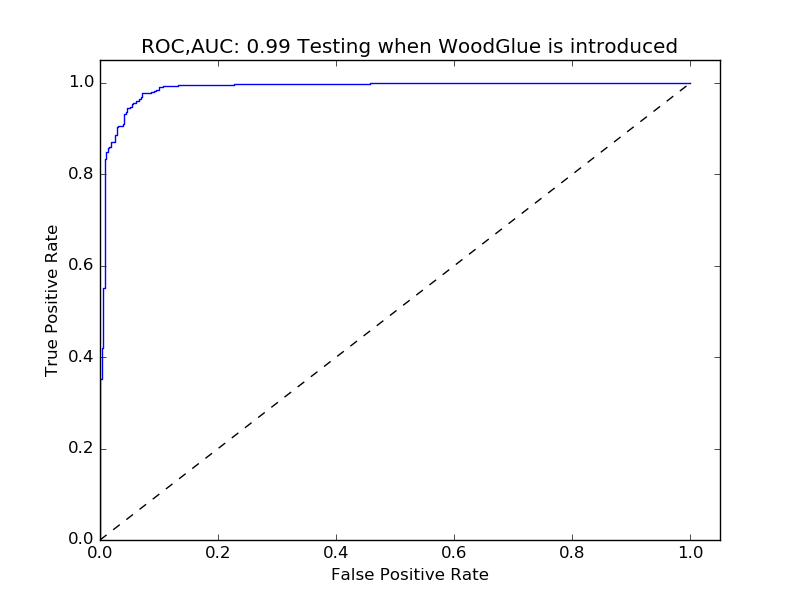
\includegraphics[width=0.5\textwidth]{/home/octopuscabbage/code/NeuralAndAdaptiveSystemsFinal/roc_curves/WoodGlue/ROC,AUC: 0.99 Testing when WoodGlue is introduced}
     }
     \caption{ROC Curves When Novel Spoofs Are Introduced}
     \label{fig-2:dummy}
   \end{figure}
   \nocite{*}

\end{document}

